\section{The sample}
\label{sec:sample}

This search covers \NWindows{} spectral windows toward \NStars{}
stars in \NSystems{} systems within 40\,pc, drawn from \NEB{}
public ALMA execution blocks and \TotalDataTB\,TB of raw data through one
frozen pipeline, \LdgCensusHours\,h on source. We call that set the
\emph{primary census}, and it is the set every limit, every crossing and
every expectation in this paper is computed over. Four further sets of blocks
enter the paper --- a hold-out reserved before the archive was searched, an
archival extension searched afterwards, an out-of-sample control beyond
40\,pc, and an external sample used only to calibrate the spatial statistic
--- and none of them is part of the primary census.
Table~\ref{tab:blockledger} gives all of them in rows that sum, with the
results each one enters; wherever a number in this paper is computed over
something other than the primary census, that table's name for it is used at
the point of use.

Three words are used consistently and are not interchangeable. A \emph{star}
is an individual stellar component; a \emph{system} is a gravitationally
bound group, counted once however many of its components were observed; a
\emph{target} is one ALMA pointing. The census holds \NStars{} stars
in \NSystems{} systems.

The census is two experiments, not one. \NWinA{} windows toward
\LdgClassAStars{} stars in \NSysClassA{} systems are fine-channel, called
\emph{Class~A} throughout: these resolve a drifting carrier and are the
primary experiment, and every sensitivity and every exclusion quoted here
refers to them unless stated otherwise. The remaining \NWinB{} windows
are coarse-channel, \emph{Class~B}, and support a secondary search for
unresolved spectral excess; they can register a spike but cannot distinguish
a drifting signal from a stationary one.

The inclusion criteria are objective and were applied by query. A star enters
if its Gaia~DR3 parallax is at least 25\,mas, measured to better than
\PlxAdqlPct{} per cent, and if its proper-motion-corrected position at the
observation epoch falls inside the quoted field of view of at least one
public execution block. Distances are direct inversions, $d=1/\varpi$, and
the star need not sit at the pointing centre. Disc, planet and spectral type
enter as descriptive metadata only, and no star or window was excluded by an
unlisted criterion or for short integration. The parallax criterion never
binds: the worst fractional parallax error among the stars searched is
\SfPlxWorstPct{} per cent, an order of magnitude inside it. The query returns
\NCensus{} work-list entries; the quoted field of view is optimistic, and
only \NGenuinelyCovered{} of those stars are in fact contained by a public
field, of which \NStars{} yielded a searchable window
(Fig.~\ref{fig:funnel}). The per-star and per-window ledger, including the
five-criterion decision tree and every edge case, is in the data release.

\subsection{The archival selection}
\label{sec:bias}

This sample was not designed. It is whatever previous ALMA programmes
happened to observe, for their own reasons, and \PctDiscProposal{} per cent
of the stars searched were targeted under a debris-disc or planet-formation
proposal. The resulting bias is strong and measurable, and
Table~\ref{tab:selfunc} tabulates it against a volume-limited reference
census selected on the same parallax quality.

\emph{The dominant selection effect is distance.} Stars within 5\,pc are
over-represented by a factor \SfTopRatio, and the enhancement falls
monotonically with distance to a factor of two \emph{under}-representation
beyond 30\,pc. Spectral type comes second: A~stars are over-represented by
about \SfARatio{} and F and G stars by factors of two to three, because those
are the stars with bright debris discs. M~dwarfs are mildly depleted ---
\SfMSearched{} of the \SfNStar{} searched stars are M~dwarfs, a factor
\SfMRatio{} of their share of the reference census, and only
\SfMClassAStars{} of them carry the fine-channel coverage that can resolve a
drifting carrier at all --- and that is a weaker
statement than the table's early-type ratios, not a stronger one. Both
figures are bounds in the same direction: Gaia temperatures are missing for
about half the reference census and missing preferentially for the coolest
objects, so the census M~fraction is a lower limit and every early-type ratio
is therefore a lower limit too. Coverage is also concentrated:
\ConcThreeWin{} of the \NWindows{} windows come from \ConcThreeSys{}
systems. Every statistical statement in this paper is therefore a statement
about an archive-selected sample of nearby stars, and none of them is an
occurrence rate for the solar neighbourhood. The systems a targeted search
would itself have chosen are collected in Table~\ref{tab:interesting}.

%% GENERATED by selfunc_v411.py -- do not hand-edit.
\begin{table}
\centering
\scriptsize
\setlength{\tabcolsep}{4pt}
\caption{Selection function of the searched sample against a volume-limited reference census, both selected on the same parallax quality: Gaia~DR3 sources with $\varpi>0$, $\sigma_\varpi/\varpi\le0.1$ and $1/\varpi\le40$\,pc (17\,566 objects, 8594 of them carrying a \texttt{teff\_gspphot} estimate), against the 89 stars with at least one searched window. The searched stars are measured far better than the cut requires --- the worst fractional parallax error among them is 2.5 per cent --- so the two columns are selected alike, and loosening the cut to 0.2 adds no census object at all. 86 of the 89 searched stars are classified: 53 from the Gaia temperature, 25 from the SIMBAD spectral type where that temperature is absent, and 8 identified as white dwarfs; 3 carry no classification in either source. The SIMBAD route matters because \texttt{teff\_gspphot} is missing preferentially for cool stars, which is the population the M~dwarf statement is about. ``Ratio'' is the sample column fraction over the census column fraction; $>1$ is over-representation. \emph{The strongest selection effect here is distance, not spectral type.}}
\label{tab:selfunc}
\begin{tabular}{@{}lrrr@{}}
\toprule
Property & Census & Searched & Ratio \\
\midrule
\multicolumn{4}{@{}l}{Distance} \\
\quad $d\le5$\,pc & 48 (0.3\%) & 12 (13.5\%) & 49.3 \\
\quad 5--10\,pc & 240 (1.4\%) & 13 (14.6\%) & 10.7 \\
\quad 10--20\,pc & 2069 (11.8\%) & 18 (20.2\%) & 1.7 \\
\quad 20--30\,pc & 5391 (30.7\%) & 19 (21.3\%) & 0.7 \\
\quad 30--40\,pc & 9818 (55.9\%) & 27 (30.3\%) & 0.5 \\
\midrule
\multicolumn{4}{@{}l}{$T_{\rm eff}$ class$^{a}$} \\
\quad A & 24 (0.3\%) & 5 (6.4\%) & 23.0 \\
\quad F & 402 (4.7\%) & 9 (11.5\%) & 2.5 \\
\quad G & 860 (10.0\%) & 16 (20.5\%) & 2.0 \\
\quad K & 1400 (16.3\%) & 7 (9.0\%) & 0.6 \\
\quad M & 5908 (68.7\%) & 41 (52.6\%) & 0.8 \\
\midrule
\multicolumn{4}{@{}l}{Other axes} \\
\quad Confirmed planet hosts$^{b}$ & 26 (15.5\%) & 23 (25.8\%) & 1.7 \\
\quad White dwarfs$^{a}$ & -- & 8 (9.0\%) & -- \\
\quad Searched stars / systems & -- & 89 / 82 & -- \\
\bottomrule
\end{tabular}

\smallskip
{\footnotesize $^{a}$Temperature bins, not MK types: A $\ge7500$, F 6000--7500, G 5300--6000, K 3900--5300, M $<3900$\,K, normalised over the 78 classified non-degenerate stars. The 8 white dwarfs are kept apart because a degenerate is not an early-type star and its photometric temperature would place it among them. Gaia \texttt{teff\_gspphot} is unavailable for about half the reference census, preferentially for the coolest and faintest objects, so the census M fraction is a lower limit and every earlier-type ratio in this panel is correspondingly a lower limit; the searched column has no such gap.\\ $^{b}$Both columns are the same positional join, of the 168-entry ALMA-covered work list and of its searched subset, to the NASA Exoplanet Archive \texttt{pscomppars} table accessed 2026 October 4; a confirmed planet is a row of that table. The 23 searched hosts carry 50 confirmed planets between them, and 21 of the 23 survive the deuterium-burning mass limit. The Gaia reference census carries no planet information, so the census column in this row is the work list rather than the 17\,566-object Gaia census.}
\end{table}


\begin{figure} \centering
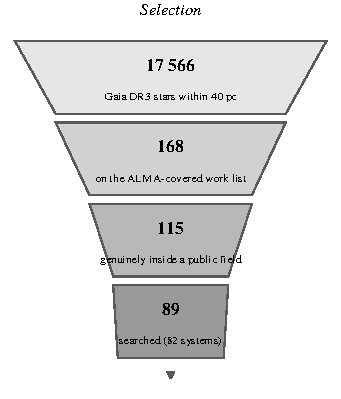
\includegraphics[width=0.66\columnwidth]{figures/selection_funnel.pdf}
\caption{The selection funnel, from the catalogued population within 40\,pc
to the stars with a searched window. The three quantities the text keeps
apart are the \NCensus-entry work list the archive query returns, the
\NGenuinelyCovered{} stars a public field genuinely contains, and the
\NStars{} that yielded a searchable window. The chain applied to what
comes out of the funnel is Fig.~\ref{fig:chain}.}
\label{fig:funnel}
\end{figure}

\subsection{Frequency coverage and archival scope}
\label{sec:coverage}

The Class~A experiment covers $\Delta\nu_A=\DnuA$\,GHz of unique sky
frequency, and that coverage is sparse: it is \DomAIslands{} disjoint islands
scattered between \DomAFreqLo{} and \DomAFreqHi\,GHz, not a band. The
endpoints are a range over which observations exist, never a range that was
covered. Adding the coarse-channel windows brings the total archival coverage
to \DnuAB\,GHz in \UnionIntervals{} intervals, of which \SearchedUnionGHz\,GHz
survives the molecular-line mask of \S\ref{sec:method}. The distribution is
shown in Fig.~\ref{fig:waterfall}; a transmitter at a frequency between the
islands was never observable here, whatever its power.

The archive is not exhausted either, and the shortfall is accounted for
rather than estimated. \LdgExtScope{} further blocks lie inside the same
query but were not processed when the census was frozen;
Table~\ref{tab:blockledger} gives what became of each. \LdgExtSearched{} of
them have since been calibrated and searched, and they enter this paper only
as repeat epochs. The largest single gap is the \FateNoCal{} blocks for which
the archive holds raw visibilities that were never pipeline-calibrated,
\FateNoCalGB\,GB in all; no effort on our side would close it.

\begin{figure*}
\centering
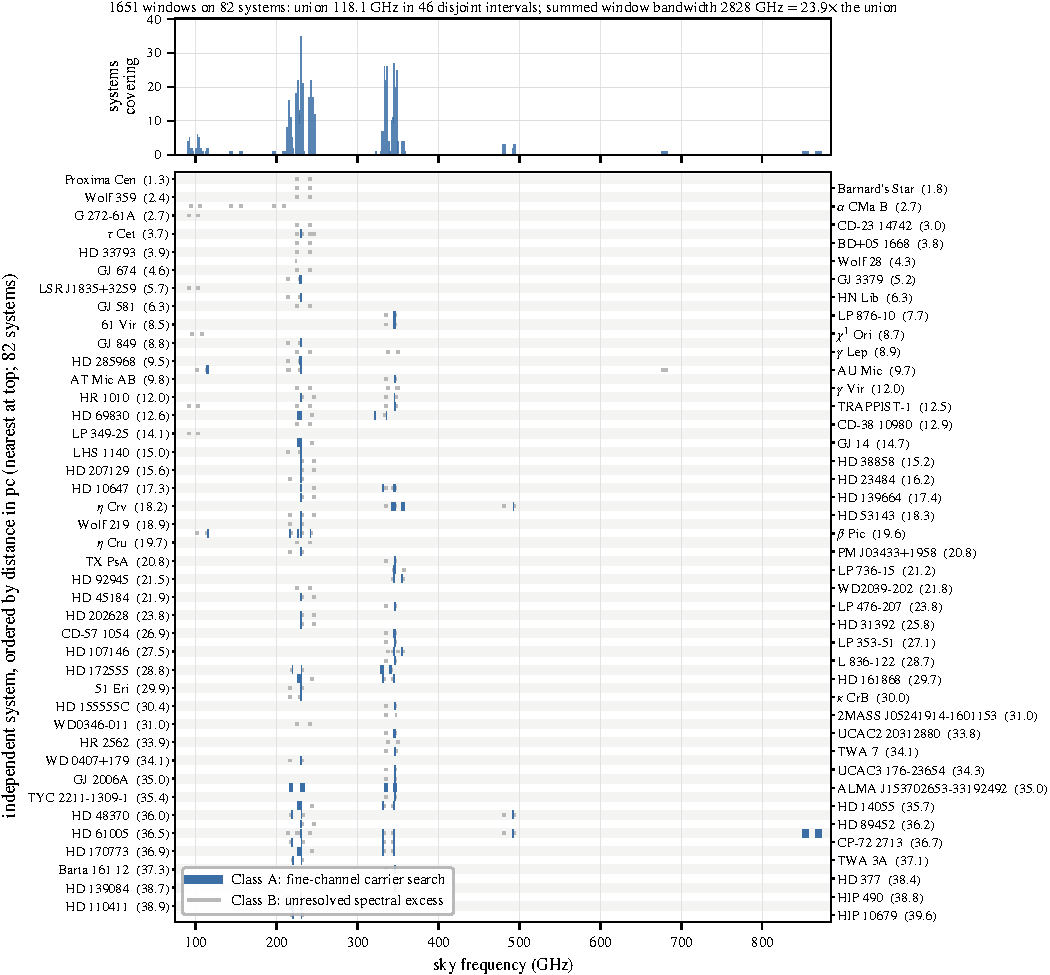
\includegraphics[width=0.99\textwidth]{figures/coverage_waterfall.pdf}
\caption{Where this survey searched. \emph{Lower panel:} each searched
window is a horizontal segment on its host system's row, rows ordered by
distance and labelled alternately on the left and right axes; heavy blue
marks the fine-channel carrier search (Class~A) and light grey the
coarse-channel spectral-excess search (Class~B). \emph{Upper panel:} the number
of systems covering each gigahertz of sky frequency; the threshold
distribution is Fig.~\ref{fig:context}(a). The coverage is narrow, clustered
and repeatedly revisited: \UnionIntervals{} islands concentrated near 230
and 345\,GHz, with summed window bandwidth $\GrossOverUnion\times$ the
union. The union measures frequency coverage, the summed bandwidth
integrated search effort.}
\label{fig:waterfall}
\end{figure*}

\begin{table*}
\centering
\scriptsize
\caption{The block and window ledger. Every set of execution blocks used
anywhere in this paper, with the results it enters; the rows sum, and each
indented group sums to the row above it. The primary census is the survey:
unless a statement names one of the other sets, it is computed over that row.
Hours are on-source hours. Confirmed planets in
Table~\ref{tab:interesting} are taken from the \SfHostCatalogue{}
\SfHostTable{} table, accessed \SfHostDate.}
\label{tab:blockledger}
%% GENERATED by blockledger_v411.py -- do not hand-edit.
\begin{tabular}{@{}p{0.285\textwidth}rrrrrp{0.275\textwidth}@{}}
\hline
Set of execution blocks & Blocks & Windows & Stars & Systems & Hours & Results it enters \\
\hline
Archival scope: blocks the query exposes & 656 & -- & -- & -- & -- & defines the scope; enters no statistic \\
Processed with the frozen pipeline & 484 & -- & -- & -- & -- & the sum of the three rows below \\
\hspace{1.1em}\textbf{Primary census} & 404 & 1651 & 89 & 82 & 1094 & every limit, the crossing list, every chance expectation \\
\hspace{2.2em}Class~A, fine channels$^{a}$ & -- & 402 & 65 & 60 & 227 & the drifting-carrier experiment \\
\hspace{2.2em}Class~B, coarse channels$^{a}$ & -- & 1249 & 88 & 81 & 867 & the spectral-excess experiment \\
\hspace{1.1em}Reserved hold-out & 77 & 315 & 36 & -- & 214 & the rank displacement, the false-alarm tail factor, the radial control profile \\
\hspace{1.1em}No window survived the quality cut & 3 & 0 & 0 & 0 & 0 & nothing \\
\hline
In scope, not processed at the freeze & 177 & -- & -- & -- & -- & the sum of the five fates below \\
\hspace{1.1em}Calibrated and searched & 144 & -- & -- & -- & -- & recurrence only; never a denominator \\
\hspace{2.2em}\textbf{Archival extension}, reported & 115 & 463 & 16 & 16 & 269 & recurrence, and the null on data the frozen pipeline had not seen \\
\hspace{1.1em}No calibration in the ALMA delivery & 18 & -- & -- & -- & -- & nothing; the archival gap \\
\hspace{1.1em}Calibration failed & 11 & -- & -- & -- & -- & nothing; the archival gap \\
\hspace{1.1em}Not attempted & 3 & -- & -- & -- & -- & nothing; the archival gap \\
\hspace{1.1em}Working disk insufficient & 1 & -- & -- & -- & -- & nothing; the archival gap \\
\hline
Beyond 40\,pc: out-of-sample control & 47 & 198 & 22 & -- & 88 & the external null; no science count \\
External calibration sample$^{b}$ & 326 & 1322 & 56 & -- & -- & the rank calibration and the positive control; no science count \\
\hline
\end{tabular}

{\footnotesize $^{a}$The two classes partition the census windows, not its blocks: 252 blocks carry a Class~A window and 389 a Class~B one, and most carry both.\\ $^{b}$Not a subset of the archival scope: it includes blocks toward stars outside the 40\,pc work list, so its blocks cannot be placed inside this ledger.}

\end{table*}

\begin{table}
\centering
\scriptsize
\caption{Systems of particular interest: every sample system within
15\,pc hosting at least one confirmed planet, ordered by distance.
$N_{\rm pl}$ is the confirmed-planet count, $N_{\rm A}$ the number of
Class~A windows, EIRP$_{90}$ the deepest Class~A sensitivity reached, and
$N_{\rm eb}$ the number of primary-census execution blocks covering the
system, so $N_{\rm eb}>1$ means repeat epochs exist within the census.
Six of these systems have no Class~A coverage and so carry no
drift-resolving limit --- the archival selection of \S\ref{sec:bias} acting
on exactly the targets a transmitter search would choose. The full target
list is in the data release.}
\label{tab:interesting}
%% GENERATED by mk_interesting.py -- do not hand-edit.
\begin{tabular}{@{}l@{~~}r@{~~}r@{~~}l@{~~}r@{~~}r@{~~}r@{}}
\hline
System & $d$ & $N_{\rm pl}$ & Bands & $N_{\rm A}$ & EIRP$_{90}$ & $N_{\rm eb}$ \\
 & (pc) & & & & (W) & \\
\hline
Proxima Cen & 1.3 & 2 & 6 & 0 & -- & 25 \\
Barnard's Star & 1.8 & 4 & 6 & 0 & -- & 3 \\
$\tau$~Cet & 3.7 & 3 & 6 & 6 & $1.7\times10^{14}$ & 8 \\
BD+05 1668 (GJ 273) & 3.8 & 2 & 6 & 0 & -- & 25 \\
HD 33793 & 3.9 & 1 & 6 & 0 & -- & 22 \\
GJ 674 & 4.6 & 1 & 6 & 0 & -- & 20 \\
HN Lib & 6.3 & 1 & 6 & 5 & $5.6\times10^{14}$ & 5 \\
GJ 581 & 6.3 & 3 & 6 & 0 & -- & 9 \\
61 Vir & 8.5 & 3 & 7 & 5 & $1.8\times10^{14}$ & 5 \\
GJ 849 & 8.8 & 2 & 6 & 6 & $9.9\times10^{14}$ & 6 \\
HD 285968 & 9.5 & 1 & 6 & 4 & $1.3\times10^{15}$ & 4 \\
AU Mic & 9.7 & 4 & 3,6,9 & 13 & $1.7\times10^{14}$ & 14 \\
TRAPPIST$-$1 & 12.5 & 7 & 3,6,7 & 5 & $2.4\times10^{14}$ & 18 \\
HD 69830 & 12.6 & 3 & 6,7 & 22 & $1.7\times10^{14}$ & 8 \\
LHS 1140 & 15.0 & 2 & 6 & 4 & $2.8\times10^{15}$ & 4 \\
\hline
\end{tabular}

\end{table}

%% v4.11 LENGTH (Ruling 4): tab:searchspace is DELETED.  Nothing cited it --
%% `labelcheck` F4 and `xrefcheck` both reported it as typeset and never
%% referenced, which is what an owner's last citation being removed looks
%% like.  Its counts of blocks, windows, stars and systems are
%% Table~\ref{tab:blockledger}'s, its frequency unions are stated in the
%% text above and drawn in Fig.~\ref{fig:waterfall}, and its channel
%% widths and drift range are in \S\ref{sec:method}.

%% REQUEST (numbers owner): tab_interesting.tex is generated by
%% referee_r9/sample/mk_interesting.py, which reads the released
%% catalogue, the frozen census, the confirmed-planet table and
%% \SelRatioRank out of the macro layer. Please adopt it into make_all.sh so
%% the table regenerates with everything else, and point its planet column at
%% r10inputs/nea_pscomppars_60pc_v411.csv (the dated NASA Exoplanet Archive
%% extract selfunc_v411.py uses) rather than at the older unique-host file,
%% so one definition of "confirmed planet" serves both tables. Two display
%% defects in it are yours, not mine: the catalogue designation of Barnard's
%% Star prints as a SIMBAD identifier with the "NAME" prefix stripped, and
%% BD+05 1668 would read better with its GJ alias beside it. Both belong in
%% star_alias.designation.
